\iffalse
\let\negmedspace\undefined
\let\negthickspace\undefined
\documentclass[journal,12pt,twocolumn]{IEEEtran}
\usepackage{cite}
\usepackage{amsmath,amssymb,amsfonts,amsthm}
\usepackage{algorithmic}
\usepackage{graphicx}
\usepackage{textcomp}
\usepackage{xcolor}
\usepackage{txfonts}
\usepackage{listings}
\usepackage{enumitem}
\usepackage{mathtools}
\usepackage{gensymb}
\usepackage[breaklinks=true]{hyperref}
\usepackage{tkz-euclide} % loads  TikZ and tkz-base
\usepackage{listings}
\usepackage{gvv}
\usepackage{circuitikz}

\newtheorem{theorem}{Theorem}[section]
\newtheorem{problem}{Problem}
\newtheorem{proposition}{Proposition}[section]
\newtheorem{lemma}{Lemma}[section]
\newtheorem{corollary}[theorem]{Corollary}
\newtheorem{example}{Example}[section]
\newtheorem{definition}[problem]{Definition}

\newcommand{\BEQA}{\begin{eqnarray}}
\newcommand{\EEQA}{\end{eqnarray}}
\newcommand{\define}{\stackrel{\triangle}{=}}
\theoremstyle{remark}
\newtheorem{rem}{Remark}

\graphicspath{./figs/}

%\bibliographystyle{ieeetr}
\begin{document}
%

\bibliographystyle{IEEEtran}


\vspace{3cm}

\title{
	%	\logo{
	Gate Assignment

	\large{EE:1205 Signals and Systems}

	Indian Institute of Technology, Hyderabad
	%	}
}
\author{Kunal Thorawade

EE23BTECH11035
}	
\maketitle


\newpage

%\tableofcontents

\bigskip
 
 \renewcommand{\thefigure}{\theenumi}
 \renewcommand{\thetable}{\arabic{table}}
 \renewcommand{\thefigure}{\arabic{figure}}
 %\renewcommand{\theequation}{\theenumi}

 \textbf{Question}:
 In the circuit shown below, the amplitudes of the voltage across the resistor and the capacitor are equal. What is the value of the angular frequency $\omega_o$ (in rad/s)? 
 (Round off the answer to one decimal place.)
 \hfill(GATE BM 32 2023)
 \begin{circuitikz}
	     % Voltage source
	     \draw (0,0) to[sV, v=$100\cos(\omega_{0} t)$] (0,2);
	         
		     % Resistor
		         \draw (0,2) to[R, l=$1\text{ k}\Omega$] (3,2);
			     
			         % Capacitor
				     \draw (3,2) to[C, l=$100\mu\text{F}$] (3,0);
				         % Ground
					     \draw (3,0) -- (0,0);
 \end{circuitikz}

 \solution
 \fi
 \begin{table}[ht]
	  \centering
	    \begin{tabular}{|c|c|c|}
		        \hline
			   \textbf{ Parameter} & \textbf{Value} & \textbf{Description} \\
			       \hline
			           $v\brak{t}$ & $100cos\brak{\omega_0 t}$ & Input Voltage \\
				       \hline
				           $R$ & $1\text{ k}\Omega$ & Resistance \\
					       \hline
					           $C$ & $100\mu\text{F}$ & Capacitance \\
						       \hline
						           $\omega_0$ & ? & Angular Frequency  \\
							       \hline
							           $Z_R = R$ & $10^3$ & Impedance for resistor  \\
								       \hline
								           $Z_C = \frac{1}{j\omega C}$ & $\frac{10^{4}}{j\omega_0}$ & Impedance for capacitor  \\
									       \hline
									           $Z = R + \frac{1}{j\omega C}$ & $10^3 + \frac{10^4}{j\omega_0}$ & Total Impedance \\
										       \hline
										         \end{tabular}
											   \vspace{2mm}
											     \caption{Parameter Table}
											       \label{BM_23_32}
\end{table}

 \begin{align}
	 R &\stackrel{\mathcal{F}}{\longleftrightarrow} R \\
	 C &\stackrel{\mathcal{F}}{\longleftrightarrow} \frac{1}{j\omega_0 C} \\
	 \abs{V_R\brak{\omega}} &= \abs{V_C\brak{\omega}} \\
	 \implies \abs{Z_R} &= \abs{Z_C} \\
	 10^3 &= \frac{10^4}{\omega_0} \\
	 \therefore \omega_0 &= 10.0
 \end{align}
 \begin{circuitikz}
	 % Voltage source
	 \draw (0,0) to[sV, v=$V(\omega)$] (0,2);
	 % Resistor
	 \draw (0,2) to[R, l=$R$, i=$I(\omega)$] (3,2);
	 % Capacitor
	 \draw (3,2) to[C, l=$\frac{1}{j\omega_0 C}$] (3,0);
	 % Ground
	 \draw (3,0) -- (0,0);
 \end{circuitikz}
 \begin{figure}[ht]
	     \centering
	         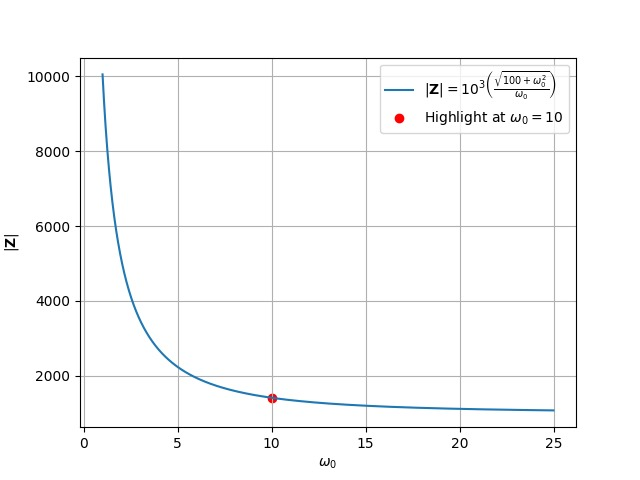
\includegraphics[width = 8cm]{2023/BM/32/figs/fig1.jpg}
		     \caption{Plot of $\abs{Z} = 10^3(\frac{\sqrt{100 + \omega_0^2}}{\omega_0}) $ }
		         \label{fig1.BM.32}
 \end{figure}
 \begin{figure}[ht]
	     \centering
	         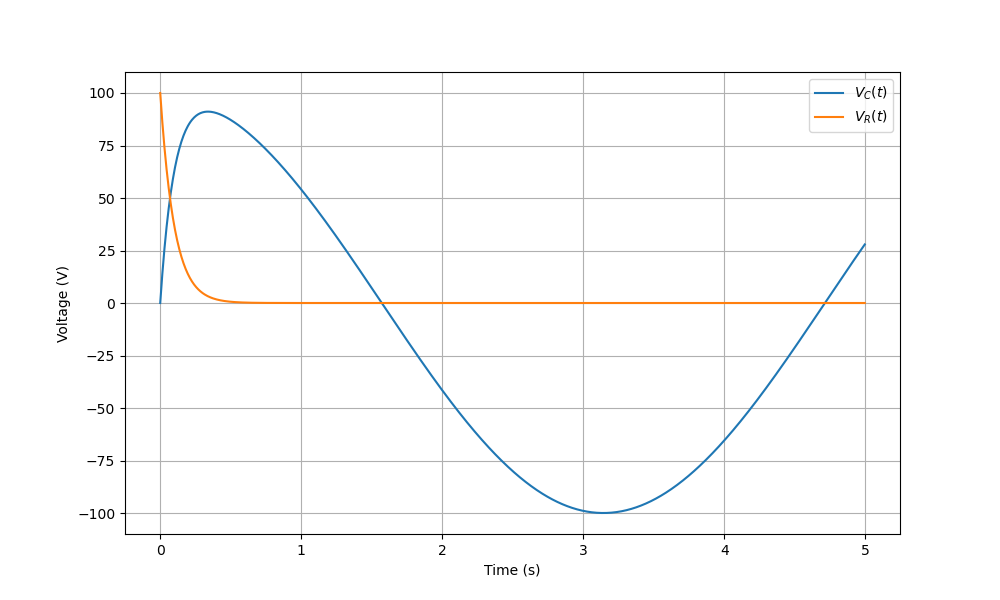
\includegraphics[width = 8cm]{2023/BM/32/figs/fig2.png}
		     \caption{Plot of Voltage Across Capacitor and Resistor}
		         \label{fig2.BM.32}
 \end{figure}
 
